% !TEX encoding = UTF-8
% !TEX TS-program = pdflatex
% !TEX root = ../tesi.tex

%**************************************************************
\chapter{Progettazione e sviluppo}
\label{cap:progettazione-sviluppo}
%**************************************************************

\intro{Il capitolo approfondisce come si è affrontato il problema, le tecnologie e le scelte fatte nel progetto.}\\

\section{Procedura di lavoro}
Il tutor aziendale si è sempre dimostrato molto disponibile durante tutta la durata dello stage. Non sono stati usati sistemi di ticketing per segnalare lo stato di avanzamento del lavoro, ma si è lavorato in maniera più informale e diretta. 

Le proposte di miglioramento (p.es. \gls{algoritmi-fonetici}) e  su come implementare (p.es. ricerche aggregate), sono state prima raccolte in un foglio su Google Doc e poi discusse di persona con il tutor.

\subsection{Individuazione del materiale}
Parte del lavoro è stata riuscire a reperire del materiale di studio adatto: tale ricerca è iniziata una settimana circa prima dell'inizio effettivo dello stage. Il materiale inizialmente ricercato riguardava la parte di:
\begin{itemize}
    \item recupero dell'informazione
    \item Javascript
\end{itemize}
sia cartaceo, che elettronico, disponibile grazie all'ateneo\footnote{\url{https://catalogo.unipd.it}}. 

\subsection{Realizzazione di un prototipo}
Dopo infarinatura iniziale degli argomenti principali di recupero dell'informazione e uno studio della libreria lunr.js, si è proceduto quindi con la realizzazione di un primo prototipo di ricerca, che consentisse la ricerca all'interno del \gls{corpus}(che sono stati convertiti in \gls{json}\glsfirstoccur{} utilizzando NodeJS). 
Al prototipo iniziale, è stato quindi aggiunto uno stemmer italiano e delle stopword: il prototipo così ottenuto è stata la base di confronto rispetto alle versioni successive (ovvero quelle che implementano l'uso di tesauri e l'analisi della semantica latente). 

\subsection{Tesauro generato manualmente}
Quindi si è passati alla realizzazione manuale di un tesauro: molto semplice dal punto di vista della programmazione (si tratta di una PipelineFunction\footnote{\url{https://lunrjs.com/docs/lunr.PipelineFunction.html}} di lunr.js che espande le interrogazioni con i sinonimi dei termini richiesti dall'utente), più difficile ed oneroso in termini di tempo dal punto di vista della compilazione del tesauro.
La strategia adottata inizialmente è stata lo studio delle frequenze dei termini e degli stem, che però si è rivelata essere infruttuosa; la strategia adottata alla fine è stata, su proposta del candidato, quella di utilizzare il modello di \gls{pos-tagger}\glsfirstoccur{} allenato da un altro tesista.

\subsection{Piano di test}
Si è allora passati alla creazione di un piano di test: tale attività sarebbe dovuta avvenire a monte della soluzione basata su tesauro costruito manualmente ma così non è stato, per la difficoltà rivelatasi nell'individuare delle interrogazioni con falsi negativi; questa inversione se non altro ha garantito che i dati del tesauro non fossero appositamente costruiti in base ai test pianificati. 

\subsection{Tesauro generato automaticamente}
La realizzazione di un tesauro automaticamente generato ha richiesto un'ulteriore approfondimento studio: sia per quanto riguarda il recupero dell'informazione che per, nello specifico, la generazione automatica di un tesauro (sia su libri di testo che su paper). La scelta di utilizzare co-occorrenze nella costruzione dei sinonimi è stata dettata dalla limitazione della dimensione del tesauro stesso:

\begin{center}
    "\textit{synonyms do not cooccur, but rather have similar cooccurrence patterns}"
\end{center}

Il tesauro così composto individua bene le parole composte (utile per la migliorare la precisione) e non i sinonimi. 

\subsection{Refactoring e tesauro generico}
Prima di integrare un tesauro generico si è proceduto a:
\begin{itemize}
    \item refactoring del codice;
    \item conversione del tesauro di LibreOffice con l'utilizzo della libreria thesaurus.
\end{itemize}

\subsection{Analisi della semantica latente}
Per poter implementare la soluzione dell'analisi della semantica latente, è stato necessario:
\begin{itemize}
    \item individuare ulteriore materiale di studio;
    \item individuare una libreria per il calcolo della \gls{svd};
    \item approfondire lo studio della libreria lunr.js.
\end{itemize}

Per quanto riguarda la parte teorica, è stato di fondamentale aiuto il tutor aziendale; per riuscire poi a implementarlo è stato necessario un approfondimento su come viene implementata la ricerca da lunr.js(leggendo il codice della libreria).

\subsection{Documentazione}
Infine, è stata realizzata la documentazione del codice, utilizzando \gls{jsdoc}.
%**************************************************************
\section{Librerie}
Fatta eccezione per lunr.js, le librerie scelte sono state proposte dal candidato; il vincolo principale era, per le librerie che avrebbero dovuto permettere la ricerca, di essere scritte in Javascript (preferibilmente eseguibili lato browser).
Nella scelta delle librerie i dei linguaggi, si è tenuto conto dei seguenti criteri:
\begin{itemize}
    \item possibilità di essere eseguita via browser;
    \item funzionalità disponibili;
    \item dipendenze;
    \item supporto e sviluppo;
    \item disponibilità di documentazione.
\end{itemize}

\subsection{Lunr.js}
%\begin{figure}
%    
\includegraphics[scale=0.15]{immagini/lunrjs-logo.jpg}
%    \caption{Logo di Lunr.js}
% \end{figure}
lunr.js è una libreria semplice da utilizzare, ma comunque potente: permette di fornire la funzionalità ricerca senza aver necessariamente bisogno di servizi esterni. 
È pensata per essere utilizzata con collezioni relativamente piccole: ciò nonostante, non trascura l'aspetto dell'efficienza (sia il costo computazionale delle operazione che lo spazio occupato in memoria). 
Non ha dipendenze esterne e può essere eseguita sia da browser che all'interno di un server Node.js.
È stata utilizzata per l'indicizzazione e per la ricerca dei documenti all'interno del \gls{corpus}.

\FloatBarrier

\subsection{LALOLib}
LALOLib (Linear ALgebra Online Library) è una libreria interamente scritta in Javascript: rende facile effettuare operazioni algebriche direttamente da browser. È eseguibile sia in modalità sincrona che asincrona. È sviluppata dal Laboratoire Lorrain de Recherche en Informatique et ses Applications come parte del progetto MLweb costituisce il core di LALOLab (un ambiente di calcolo scientifico online). È anche alla base di ML.js, una libreria in Javascript library per il machine learning. 
LALOLib include funzioni per:
\begin{itemize}
    \item algebra lineare;
    \item statistica;
    \item ottimizzazione (con glpk.js);
    \item machine learning (con ML.js).
\end{itemize}

La scelta della libreria è stata vincolata, a causa della scarsità di librerie di calcolo scientifico in Javascript che siano al contempo attivamente sviluppate e che supportino il calcolo della \gls{svd} (p.es. tensorflow.js\footnote{\url{https://github.com/tensorflow/tfjs/issues/110}} allo stato attuale non lo permette e sushi2\footnote{\url{https://github.com/mil-tokyo/sushi2}} non è più sviluppata da quasi 3 anni) 

È stata utilizzata per effettuare i calcoli matriciali necessari allo sviluppo del tesauro automaticamente generato(i.e. il calcolo della matrice delle similarità) e per l'analisi della semantica latente.


\subsection{NumPy}
NumPy è una libreria open source per il linguaggio di programmazione Python, che aggiunge supporto a grandi matrici e array multidimensionali insieme a una vasta collezione di funzioni matematiche di alto livello per poter operare efficientemente su queste strutture dati. È stato creato nel 2005 da Travis Oliphant basandosi su Numeric di Jim Hugunin. È stato utilizzato come confronto delle performance della libreria LALOLib nel calcolo della decomposizione ai valori singolari della matrice termini-documenti normalizzata (necessario per l'analisi della semantica latente). In particolare, fa uso della routine \texttt{\_gesdd} della libreria LAPACK (scritta in Fortran) per il calcolo della \gls{svd}; è stata scelta questa libreria e non SciPy come termine di confronto in quanto entrambe non sfruttano la sparsità della matrice nel calcolo della \gls{svd}.

\subsection{scikit-learn}
Scikit-learn è una libreria open source di apprendimento automatico per il linguaggio di programmazione Python, progettata per operare con le librerie NumPy e SciPy: è stata scelta dal candidato per prendere familiarità inizialmente con il dominio (recupero dell'informazione).

\subsection{OpenNLP}
Apache OpenNLP è una libreria per l'elaborazione del linguaggio naturale facendo uso del machine learning.
Supporta, per esempio, il riconoscimento del linguaggio, tokenization, POS tagging, chunking e molto altro. È stata utilizzata per il POS tagging, utilizzando un modello allenato da un altro tesista\footnote{Jiancheng Ye, laureando in Ingegneria Informatica presso l'Università degli Studi di Padova}.

\subsection{Riepilogo}
 Un riepilogo delle librerie utilizzate, per linguaggio e scopo.
 \begin{center}
    \begin{tabular}{p{0.15\linewidth}lp{0.5\linewidth}}
        \toprule
        Linguaggio & Libreria & Scopo \\
        \midrule
          Javascript (browser) & lunr.js & Indicizzare i documenti, filtrare alcuni termini irrilevanti al fine delle ricerche tramite stopword, configurare uno stemmer, effettuare le ricerche sull'indice creato e quindi ritornare i documenti recuperati in base al loro score. \\
           & LALOLib & Effettuare i calcoli matriciali necessari per la generazione automatica di un tesauro (i.e. calcolo della matrice delle similarità) e per l'analisi della semantica latente (i.e. \gls{svd}, moltiplicazioni tra matrici) \\
           \addlinespace
          NodeJS &  srt-to-json & Convertire i file delle trascrizioni in un JSON rappresentante il \gls{corpus} dei documenti. \\
                 &  thesaurus & Convertire il tesauro generico di LibreOffice in JSON, per permettere il suo utilizzo all'interno del progetto.\\
        \addlinespace
          Python & NumPy        & Confronto delle performance del calcolo della decomposizione ai valori singolari \\
                 & scikit-learn & Studio iniziale del recupero dell'informazione.\\
        \addlinespace
          Java   & OpenNLP      & Taggare i termini in base alla parte del discorso. (per il tesauro generato manualmente)\\
        \bottomrule
    \end{tabular}
        \captionof{table}[Riepilogo librerie]{Librerie utilizzate durante lo stage} 
        \label{tab:librerieUsate}
    \end{center}
\newpage
\section{Indicizzazione}
\begin{figure}
    \centering
    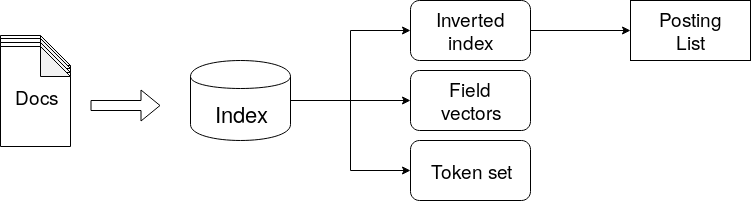
\includegraphics[scale=0.42]{immagini/indice.png}
    \caption{Indice}
    \label{fig:indice}
\end{figure}
    
La struttura dell'indice rispecchia quella impostata dalla libreria lunrjs. L'indice è dotato quindi di:
\begin{itemize}
    \item inverted index, che permette di conoscere la posting list per ogni token;
    \item field vectors, ovvero la rappresentazione interna dei documenti (come sparse vector);
    \item token set, i token presenti nei documenti, rappresentati come una macchina a stati finiti.
\end{itemize}
 
I calcoli matriciali, necessari per la generazione automatica del tesauro e per l'analisi della semantica latente, utilizzano la libreria LALOLib e non sfruttano la sparsità. (perché non si sono trovate libreria in Javascript che calcolino la \gls{svd} e sfruttino la sparsità) 

%*************************************************************
\begin{figure}
    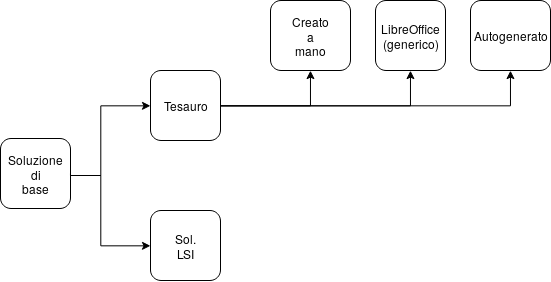
\includegraphics[scale=0.6]{immagini/schema-soluzione.png}
    \caption{Schema del prodotto}
    \label{fig:schemaProdotto}
 \end{figure}


%*************************************************************
\section{Tesauro manuale}
Per la creazione manuale di un tesauro si è fatto uso del \gls{pos-tagger} di OpenNLP: il modello italiano è basato su quello del dott. Andrea Ciapetti\footnote{\url{https://github.com/aciapetti/opennlp-italian-models}} ed era stato ulteriormente allenato da un altro tesista, fino a raggiungere dei risultati molto buoni nei test. Il \gls{pos-tagger} ha permesso di ridurre notevolmente il numero di termini da considerare, limitato ai soli verbi e sostantivi.

L'idea iniziale invece era stata quella di ordinare i termini per frequenza (sia presi singolarmente che aggregati per stem) e, dopo aver filtrato tramite stopword, cercare a mano possibili sinonimi: il numero di termini presenti presenti (1956), nonostante le stopword, si è rivelato comunque essere eccessivo. Questo approccio ha però permesso di evidenziare problematiche nella precision riguardanti i termini più frequenti; mentre ricercare i termini meno frequenti ha permesso di individuare meglio alcuni errori di trascrizione del video.

Un approccio aggiuntivo (non di immediata applicazione) poteva essere un misto tra \gls{pos-tagger} e IDF, limitando la ricerca quindi ai termini non uniformemente distribuiti nel \gls{corpus} e ai soli verbi e sostantivi.

%**************************************************************
\section{Tesauro automaticamente generato}
\label{sec:comeGenerareTesauroAuto}

    \begin{figure}
        \centering
        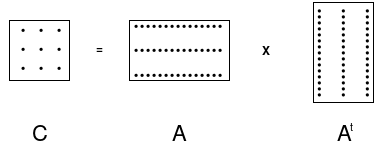
\includegraphics[scale=0.55]{immagini/calcoloSimilarita.png}
        \caption{Calcolo della matrice delle similarità}
        \label{fig:calcoloSimilarità}
     \end{figure}    

Il tesauro è stato generato in maniera automatica, calcolando le co-occorrenze dei termini.
Per fare ciò:
\begin{itemize}
    \item si crea la matrice termini-documenti $A$;
    \item si normalizza la matrice (nel caso specifico si è utilizzato TF-IDF);
    \item si calcola la matrice delle similarità $C = AA^{T}$.
\end{itemize}

Il valore dell'elemento in posizione $C_{i,j}$ della matrice è il valore della similarità tra il termine \textit{i} e il termine \textit{j}.

Si è dovuto quindi determinare una certa soglia oltre la quale i due termini \textit{i} e \textit{j} possono essere considerati simili: la scelta di tale soglia è stata puramente empirica.

%**************************************************************
\section{Latent Semantic Indexing}
\label{comeLSI}
Latent Semantic Indexing (chiamata anche Latent Semantic Analysis) è una tecnica di elaborazione del linguaggio naturale che analizza le relazioni tra un insieme di documenti e di termini che sono contenuti producendo un insieme di concetti legati ai documenti e ai termini. (si veda §\ref{cap:latent-semantic-indexing})

Ai fini del recupero dell'informazione, per semplicità di implementazione, si è deciso di utilizzare la matrice $A_k$: nel caso di un \gls{corpus} grande questo costituirebbe un fattore limitante, ma si è visto che il collo di bottiglia, nella particolare applicazione completamente lato client, è dato invece dal calcolo della decomposizione.

A livello pratico, quindi:
\begin{itemize}
    \item si crea la matrice termini-documenti $A$;
    \item si normalizza la matrice (nel caso specifico si è utilizzato TF-IDF);
    \item si decompone la matrice originale nelle matrici $U$, $S$, $V$ e si calcola $A_k$;
    \item si aggiorna la rappresentazione dei documenti sostituendola con $A_k$;
    \item si aggiorna l'indice inverso (considerando come presente solo i termini oltre una certa soglia).    
\end{itemize}

La scelta del rango(ovvero il numero di concetti) e della soglia oltre la quale considerare un termine è stata, ancora una volta, empirica.

%**************************************************************
\section{Documentazione}
Per produrre la documentazione per lo sviluppatore, si è scelto di utilizzare il tool \gls{jsdoc}, sia per la sua semplicità che per continuità con lunr.js, la libreria principalmente utilizzata. Data la semplicità di utilizzo, non c'è stata necessità di produrre della documentazione per l'utente.